\documentclass{beamer}

\mode<presentation> {
%\usetheme{default}
%\usetheme{AnnArbor}
%\usetheme{Antibes}
%\usetheme{Bergen}
%\usetheme{Berkeley}
%\usetheme{Berlin}
%\usetheme{Boadilla}
%\usetheme{CambridgeUS}
%\usetheme{Copenhagen}
%\usetheme{Darmstadt}
%\usetheme{Dresden}
%\usetheme{Frankfurt}
%\usetheme{Goettingen}
%\usetheme{Hannover}
%\usetheme{Ilmenau}
%\usetheme{JuanLesPins}
%\usetheme{Luebeck}
\usetheme{Madrid}
%\usetheme{Malmoe}
%\usetheme{Marburg}
%\usetheme{Montpellier}
%\usetheme{PaloAlto}
%\usetheme{Pittsburgh}
%\usetheme{Rochester}
%\usetheme{Singapore}
%\usetheme{Szeged}
%\usetheme{Warsaw}

% As well as themes, the Beamer class has a number of color themes
% for any slide theme. Uncomment each of these in turn to see how it
% changes the colors of your current slide theme.

%\usecolortheme{albatross}
%\usecolortheme{beaver}
%\usecolortheme{beetle}
%\usecolortheme{crane}
%\usecolortheme{dolphin}
%\usecolortheme{dove}
%\usecolortheme{fly}
%\usecolortheme{lily}
%\usecolortheme{orchid}
%\usecolortheme{rose}
%\usecolortheme{seagull}
%\usecolortheme{seahorse}
%\usecolortheme{whale}
%\usecolortheme{wolverine}

%\setbeamertemplate{footline} % To remove the footer line in all slides uncomment this line
%\setbeamertemplate{footline}[page number] % To replace the footer line in all slides with a simple slide count uncomment this line

%\setbeamertemplate{navigation symbols}{} % To remove the navigation symbols from the bottom of all slides uncomment this line
}

\usepackage{graphicx} % Allows including images
\usepackage{booktabs} % Allows the use of \toprule, \midrule and \bottomrule in tables
\usepackage{algpseudocode}
\usepackage{pifont}
\usepackage[]{algorithm2e}

%----------------------------------------------------------------------------------------
%	TITLE PAGE
%----------------------------------------------------------------------------------------

\title[Short title]{Wolf and Hare} % The short title appears at the bottom of every slide, the full title is only on the title page

\author{Nils Kohl, Thomas Stadelmayer, David Uhl} % Your name
\institute[FAU] % Your institution as it will appear on the bottom of every slide, may be shorthand to save space
{
Friedrich-Alexander Universit\"at Erlangen-N\"urnberg \\ % Your institution for the title page
\medskip
}
\date{03.07.2015} % Date, can be changed to a custom date

\begin{document}

\begin{frame}
\titlepage % Print the title page as the first slide
\end{frame}

\begin{frame}
\frametitle{Overview} % Table of contents slide, comment this block out to remove it
\tableofcontents % Throughout your presentation, if you choose to use \section{} and \subsection{} commands, these will automatically be printed on this slide as an overview of your presentation
\end{frame}

%----------------------------------------------------------------------------------------
%	PRESENTATION SLIDES
%----------------------------------------------------------------------------------------

%------------------------------------------------
\section{Wolf and Hare}
\subsection{Spielregeln}
\begin{frame}
\frametitle{Spielregeln}
\begin{itemize}
\item 2D Spielfeld mit zwei W\"olfen und einem Hasen
\item Zuf\"allige Startposition auf Spielfeld
\item Pro Zug: W\"olfe jeweils einen Schritt, Hase einen Schritt
\item Spielende: Wolf f\"angt Hasen oder Hase erreicht Ziel
\end{itemize}
\begin{block}{Aufgabe}
\begin{itemize}

\item Spiel parallelisieren
\item Jede Maschine auf Cluster testet verschiedene Routen
\end{itemize}

\end{block}
\end{frame}
 
%------------------------------------------------
\subsection{Visualisierung}
\begin{frame}
\frametitle{Visualisierung (1)}
\begin{columns}[c] % The "c" option specifies centered vertical alignment while the "t" option is used for top vertical alignment

\column{.45\textwidth} % Left column and width
\begin{table}
\begin{tabular}{l l}
\toprule
\textbf{x-Position} & \textbf{y-Position}\\
\midrule
 0 & 0 \\
0 & 1 \\
0 & 2 \\
0 & 3 \\
0 & 4 \\
1 & 4 \\
2 & 4 \\
3 & 4 \\
4 & 4 \\
\bottomrule
\end{tabular}
\caption{Wolf1}
\end{table}

\column{.5\textwidth} % Right column and width
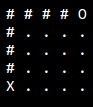
\includegraphics[scale=1,natwidth=610,natheight=642]{wolf_route_bsp.png}
\end{columns}

\end{frame}

\begin{frame}
\frametitle{Visualisierung (2)}
\begin{columns}[c] % The "c" option specifies centered vertical alignment while the "t" option is used for top vertical alignment

\column{.5\textwidth} % Right column and width
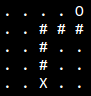
\includegraphics[scale=1,natwidth=610,natheight=642]{wolf_route.png}\\
RouteX Wolf1

\column{.5\textwidth} % Right column and width
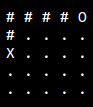
\includegraphics[scale=1,natwidth=610,natheight=642]{hare_route.png}\\
Route Hase
\end{columns}
\end{frame}

\begin{frame}

\frametitle{Visualisierung (3)}
\begin{columns}[c] % The "c" option specifies centered vertical alignment while the "t" option is used for top vertical alignment

\column{.45\textwidth} % Left column and width
\begin{table}
\begin{tabular}{l l}
\toprule
\textbf{x-Position} & \textbf{y-Position}\\
\midrule
 0 & 0 \\
1 & 0 \\
2 & 0 \\
3 & 0 \\
4 & 0 \\
4 & 1 \\
4 & 2 \\
4 & 3 \\
4 & 4 \\
\bottomrule
\end{tabular}
\caption{RouteX von Wolf1}
\end{table}

\column{.5\textwidth} % Right column and width
\begin{table}
\begin{tabular}{l l}
\toprule
\textbf{x-Position} & \textbf{y-Position}\\
\midrule
 0 & 2 \\
0 & 3 \\
0 & 4 \\
1 & 4 \\
2 & 4 \\
3 & 4 \\
4 & 4 \\
4 & 4 \\
4 & 4 \\
\bottomrule
\end{tabular}
\caption{RouteX von Hase}
\end{table}
\end{columns}

\end{frame}

\section{Implementierung}
\subsection{Seriell}

\begin{frame}
\frametitle{Seriell}
\begin{itemize}
\item Routenerstellung für die W\"lfe und den Hasen
\item Kombination der Wolfsrouten zu Routenpaaren
\item Unabh\"angiger Task: Vergleich eines Routenpaares mit allen Routen des Hasens
\item Speicherung der Erfolge bzw. Misserfolge des Routenpaares für alle Hasenrouten
\item Vergleich aller Routenpaare
\end{itemize}
\end{frame}



\begin{frame}
\begin{algorithm}[H]
\frametitle{Seriell}
% \KwData{this text}
% \KwResult{how to write algorithm with \LaTeX2e }
% initialization\;
\For{(w1, w2) in wolf\_routes} {
 \For{h in hare\_routes}{
   /* test if a wolf catches the hare before it arrives at the special square */
   compare (w1, w2) with h;
    
  \Comment{compares each element}\;
  \Comment{counter++}\;

  \eIf{caught}{
   append number of steps needed to list\;
   }{
   add flag to list (e.g. -1)\;
  }
 }
 }
% \caption{How to get the best routes}
\end{algorithm}
\end{frame}

\subsection{Parallel}
\begin{frame}
\frametitle{Parallel}
\begin{itemize}
\item Tupel von einer Route Wolf1 und Wolf2
\item Vergleiche Tupel mit allen Routen von Hase
\item Merke Anzahl der Schritte und Wahrscheinlichkeit als Indikatoren
\item Wenn ein Tupel mit besseren Indikatoren gefunden wird, dann l\"osche alle alten Werte und f\"uge Tupel in Liste ein

\item Tupel auf Prozessoren aufteielen
\item Nach Berechnung vergleiche die Listen
\end{itemize}
\end{frame}

\begin{frame}
\begin{algorithm}[H]
\frametitle{Parallel}
% \KwData{this text}
% \KwResult{how to write algorithm with \LaTeX2e }
% initialization\;
 $<$r1w1,r2w2$>$  = choose tupel of routes wolf1 and wolf2\;
 \For{all hare routes}{
  compare tupel with route\_i of hare\;
  \Comment{compares each element}\;
  \Comment{in case of success probability\_local++}\;
 }
 \parskip 12pt
 \noindent\hspace*{50mm} .\\
 \noindent\hspace*{50mm} .\\
 \noindent\hspace*{50mm} .\\
\end{algorithm}
\end{frame}

\begin{frame}
\begin{algorithm}[H]
\frametitle{Parallel}
% \KwData{this text}
% \KwResult{how to write algorithm with \LaTeX2e }
% initialization\;
  \If{probability\_local $<$ probability\_global}{
  	probability\_global = probability\_local\;
  	delete all elements in list\;
  	add $<$r1w1, r2w2$>$ to list\;  
   }
   \If{p\_local $==$ p\_global AND counter\_local $<$ counter\_global}{
  	counter\_global = counter\_local\;
  	delete all elements in list\;
  	add $<$r1w1, r2w2$>$ to list\;  
   }
   \If{p\_local $==$ p\_global AND counter\_local $==$ counter\_global}{
  	add $<$r1w1, r2w2$>$ to list\;  
   }
 \caption{How to get best routes}
\end{algorithm}
\end{frame}

\begin{frame}
\frametitle{Parallel}
\begin{itemize}
\item Sammle alle p\_global und counter\_global (MPI-Allgather)
\item Root: entscheide welcher Rank die besten Werte hat
\item Teile jedem Rank mit ob er die besten hat (1) oder nicht (0) (MPI-Broadcast)
\item Jeder Rank, der eine 1 erhalten hat, sendet seine ermittelten Routen zu root (MPI-Send)
\end{itemize}
\end{frame}

\end{document} 
